\documentclass[10pt,conference]{IEEEtran}
\IEEEoverridecommandlockouts
% The preceding line is only needed to identify funding in the first footnote. If that is unneeded, please comment it out.
%\usepackage{cite}
\usepackage{amsmath,amssymb,amsfonts}
\usepackage{algorithmic}
\usepackage{graphicx}
\usepackage{textcomp}
\usepackage{xcolor}
\usepackage{newtxmath}
\usepackage{hhline}

\usepackage[style=ieee, sortcites=true, sorting=none, urldate=iso,date=iso,seconds=true]{biblatex}
\addbibresource{bibliography.bib}

%\usepackage{acronym}

%\newacronym{6DoF}{6DoF}{Six Degrees of Freedom}

\def\BibTeX{{\rm B\kern-.05em{\sc i\kern-.025em b}\kern-.08em
    T\kern-.1667em\lower.7ex\hbox{E}\kern-.125emX}}

    % Source - https://tex.stackexchange.com/a/609374
% Posted by moewe
% Retrieved 2026-10-27, License - CC BY-SA 4.0

%\renewcommand*{\bibfont}{\normalfont\small}
\AtBeginBibliography{\small}

\begin{document}

% General Variables
\newcommand{\g}{\ensuremath{\mathbf{g}}} % Gravitational Acceleration
\newcommand{\J}{\ensuremath{\mathbf{J}}} % Inertial Matrix

% Defender Variables
\newcommand{\xD}{\ensuremath{\mathbf{x}}} % State Vector
\newcommand{\pD}{\ensuremath{\mathbf{p}}} % Position
\newcommand{\vD}{\ensuremath{\mathbf{v}}} % Translational Velocity
\newcommand{\dcmD}{\ensuremath{\mathbf{A}}} % Rotation Matrix
\newcommand{\wD}{\ensuremath{\mathbf{w}}} % Angular velocity
\newcommand{\uD}{\ensuremath{\mathbf{u}}} % Control Input

% Attacker Variables
\newcommand{\xA}{\ensuremath{\mathbf{z}}} % State Vector
\newcommand{\pA}{\ensuremath{\mathbf{d}}} % Position
\newcommand{\vA}{\ensuremath{\mathbf{s}}} % Translational Velocity
\newcommand{\dcmA}{\ensuremath{\mathbf{R}}} % Rotation Matrix
\newcommand{\wA}{\ensuremath{\mathbf{o}}} % Angular velocity

% Reachability Variables
\newcommand{\ED}{\ensuremath{\Phi}} % Defender Reachable Set at time k
\newcommand{\EA}{\ensuremath{\Psi}} % Attacker Reachable Set at time k
\newcommand{\RD}{\ensuremath{\mathcal{D}}} % Defender Reachability Cone (set of reachable sets at k=0:N)
\newcommand{\RA}{\ensuremath{\mathcal{A}}} % Attacker Reachability Cone (set of reachable sets at k=0:N)
\newcommand{\RS}{\ensuremath{\mathcal{S}}} % Safe Reachability Cone
\newcommand{\ES}{\ensuremath{\Upsilon}} % Safe Reachable Set

% Parametope Variables
\newcommand{\alphaD}{\ensuremath{\mathbf{\alpha}}} % Defender Parameter Matri
\newcommand{\yD}{\ensuremath{y}} % Defender Squared Radius
\newcommand{\alphaA}{\ensuremath{\mathbf{\gamma}}} % Attacker Parameter Matri
\newcommand{\yA}{\ensuremath{r}} % Attacker Squared Radius

% Commands
\newcommand{\vm}[1]{%
%  \ifstrequal{#1}{\omega}{\boldsymbol{#1}}{%
%    \ifstrequal{#1}{\tau}{\boldsymbol{#1}}{\mathbf{#1}}
%  }
\ensuremath{\mathbf{#1}}
} % Vector or matrix (only works on text)

\newcommand{\KLD}[2]{\ensuremath{\kappa(#1,#2)}} % KLD function
\newcommand{\bKLD}[2]{\ensuremath{K(#1,#2)}} % big KLD function

\newcommand{\LSE}[1]{\ensuremath{l (#1)}} % LSE function

\newcommand{\ellip}[2]{\ensuremath{\varepsilon (#1,#2)}}

\newcommand{\so}[1]{[#1]_{\times}} % Skew Asymmetric matrix

\title{Autonomous UAV Control in Adversary Scenarios: An Application of Reachability Analysis via Controlled Dynamical Embeddings\\
%{\footnotesize \textsuperscript{*}Note: Sub-titles are not captured in Xplore and
%should not be used}
}

\author{\IEEEauthorblockN{António Canteiro}
\thanks{*This work was not supported by any organization}% <-this % stops a space
\thanks{$^{1}$Albert Author is with Faculty of Electrical Engineering, Mathematics and Computer Science,
        University of Twente, 7500 AE Enschede, The Netherlands
        {\tt\small albert.author@papercept.net}}%
\thanks{$^{2}$Bernard D. Researcheris with the Department of Electrical Engineering, Wright State University,
        Dayton, OH 45435, USA
        {\tt\small b.d.researcher@ieee.org}}%
}


\maketitle

\begin{abstract}
%State the Problem: Guarantee area defense in a reach-avoid scenario with quad-rotor UAVs.\\
%Why is it an interesting problem: If the set of possible defender trajectories fully intersects the set of attacker trajectories at some moment in the future, then interception is assured and area defense is guaranteed.\\
%What my solution achieves: novel MPC based strategy which drives the dynamically modelled defender reachable set to overlap the attacker reachable set.\\
%What follows from my solution: The defender continuously maneuvers itself to the trajectory most likely to reach all possible attacker trajectories.

In a reach-avoid scenario in which a quad-rotor UAV is preventing an attacking UAV from reaching a critical area, the defender must be guaranteed to reach the attacker before the attacker reaches the critical area.

%This is especially true in the real world, where ensuring area defense against potentially hostile UAVs is paramount.

Expanding on previous work on defensive control strategies for reach-avoid games, this thesis proposes a novel NMPC based strategy which drives the set of possible defender trajectories to overlap with the set of possible attacker trajectories. Unlike other NMPC and CBF based strategies, the set of possible trajectories is continuously updated according to the quad-rotor dynamics.

With the proposed control strategy, the defender continuously maneuvers itself to the trajectory most likely to reach all possible attacker trajectories, thus maintaining a guarantee of area defense throughout its operational period.

%A preventative solution to unauthorized incursions of commercial drones into urban airspaces lies in autonomous quad-rotor UAV control in area defense scenarios. 

%Previous MPC solutions enforce conditions on the defender trajectory through barrier constraints that guarantee it intercepts the attacker before the attacker reaches its target. These constraint-based solutions, however, may fall into mathematical infeasibility and fail to pursue their goal. 

%This dissertation proposes a novel NMPC based solution which sidesteps the infeasibility problem and offers a best-possible defense strategy by defining the objective function as a scalar-valued continuous function that represents an area defense score, using parametric reachable set analysis and ellipsoidal calculus.

%The effectiveness of the proposed controller in several reach-avoid scenarios is demonstrated by computer simulations which show that the defender can reliably block the attacker's feasible trajectories to its target. Additionally, the notion of a "safeguarded area" is introduced, which measures the overlap between the defender and attacker reachable sets.\\
\end{abstract}

\begin{IEEEkeywords}
quad-rotor, UAV, reach-avoid, control, autonomous, adversarial, NMPC, reachability, embeddings, defense
\end{IEEEkeywords}

\section{Introduction}
Unauthorized drone flights into airport airspaces are an increasingly pressing and disruptive issue, as reported by Euronews~\cite{newsDronesAirports}, and to prevent closures, autonomous quad-rotor UAV control has been proven to be an effective strategy for direct and early prevention of airspace trespassing~\cite{WATKINSdrones}.

This scenario of autonomous area defense/target pursuit can be formulated as a reach-avoid game, as outlined in the seminal work~\cite{isaacs1999differential_seminal}. These games pose a control problem which have been addressed through optimal control strategies, which require solving the computationally expensive Hamilton-Jacobi-Isaacs equation~\cite{zhou2016cooperative}~\cite{hayoun2017guaranteeing}, but suboptimal strategies such as system decomposition provide computationally tenable solutions~\cite{Bui2025ReachAvoidDG}. MPC based approaches provide reach-avoid trajectory planning by coupling the dynamics of adversarial players in the penalty function~\cite{DoraN}, and CBF based strategies can assure defense conditions, but only while feasible~\cite{LiB}, and are limited to Lyapunov functions~\cite{AliMPCCBF}~\cite{davydov2021pursuer}~\cite{chen2025cooperative}.

This work tackles the problem of ensuring area defense in a reach-avoid scenario between a defender UAV and an unpredictable attacker UAV, and aims to expand on the control approaches proposed previously. As contributions, this work proposes: 1) the safe reachability cone as a tool to validate a defensive trajectory, presented in Section~\ref{sec:safe-reachability-cone}; and 2) an MPC based defense strategy that ensures the defender reachability cone overlaps the attacker reachability cone for as long as possible, presented in Section~\ref{sec:defense-controller-formulation}. 

It is organized as follows: firstly in Section~\ref{sec:attacker-defender-scenario} the quad-rotor model to be used is defined, followed by the mathematical formulation of the reach-avoid problem to address. Then in Section~\ref{sec:parametric-reachable-set} the quad-rotor parametric reachable set representation is defined, as well as the reachability cone for both defender and attacker. The safe reachability cone, an auxiliary tool used to validate defensive strategies, is defined in Section~\ref{sec:safe-reachability-cone}. The MPC based defense strategy is developed in Section~\ref{sec:defense-controller-formulation}, utilizing the reachability cones. Finally, in Section~\ref{sec:simulations-and-discussion} the effectiveness of the proposed control strategy is shown in a simulated environment. Conclusionary remarks and suggestions of future work are presented in Section~\ref{sec:conclusions-and-further-work}.\\

%This thesis tackles the specific problem of area defense using a defending quad-rotor UAV against an unpredictable attacking drone. The defender is successful if the set of possible defender trajectories fully intersects the set of attacker trajectories at some moment in the future, at which point interception is assured and area defense is guaranteed.\\

\paragraph*{Notation} 
\par The set of real numbers is denoted by $\mathbb{R}$. The identity matrix is denoted by $\mathbb{I}$. Given a vector $\vm{v} \in \mathbb{R}^n$, its transpose is denoted by $\vm{v}^T$, and likewise for a matrix $\vm{M}$. The inner product between two matrices or vectors is denoted by $\vm{v} \cdot \vm{M}$. The cross product operation between a vector and a matrix, denoted by $\vm{v} \times \vm{M}$, is equivalent to the inner product between the skew asymmetric matrix ($SO(3)$) of that vector, which is denoted by $\so{\vm{v}}$, and that matrix. When applied to a matrix, $\so{\vm{M}}$, it can also be used to represent the inverse transformation from an $SO(3)$ matrix to an $\mathbb{R}^3$ vector. The operation vec($\vm{M}$) returns the vectorized matrix.

\section{Attacker-Defender Problem Formulation}
\label{sec:attacker-defender-scenario}
The conditions of the reach-avoid scenario are firstly formulated, starting with the definition of the quad-rotor model in Subsection~\ref{ssec:quad-rotor-model}. This is followed, in Subsection~\ref{ssec:area-defense}, by the definition of the attacker's goal and the conditions the defender must satisfy.

The scenario in study is a reach-avoid game between a defender drone and an attacker drone. The attacker's goal is to reach a critical area, and it may take any feasible trajectory that accomplishes this goal in reasonable time. The defender's goal is to reach the attacker before it reaches the critical area, despite the exact attacker trajectory not being known ahead of time. The challenge lies in ensuring that the set of possible defender trajectories fully intersects with the set of attacker trajectories at some moment in the future, thus ensuring the defender reaches the attacker and guaranteeing area defense.

\subsection{Quad-Rotor Model}
\label{ssec:quad-rotor-model}
The quad-rotor drone 6DoF model is built on the assumptions that its mass remains constant, the method of propulsion are four vertical rotors, attitude control is provided by a torque vector and altitude control by a scalar thrust input, it has GNC capability that allows it to discern its position relative to obstacles and the target and path plan, and it is subject to aerodynamic drag. The model is based on the Euler-Angle-Free model described in~\cite{AssloujE}.

The control input to the quad-rotor drone model can be written as $\uD \in \mathbb{R}^4$ where $u_1$ is the net body force and $u_2$, $u_3$, $u_4$ are the body moments. The position $\pD \in \mathbb{R}^3$ dynamics is defined by the equation
\begin{equation}
    \dot{\pD} = \vD,
\end{equation}
and the velocity $\vD \in \mathbb{R}^3$ dynamics by the equation
\begin{equation}
    \dot{\vD} =  \g + \frac{u_1}{m} \dcmD \cdot \vm{e}_{z}.
\end{equation}
The rotation matrix $\dcmD \in \mathbb{R}^{3 \times 3}$ dynamics are expressed by
\begin{equation}
    \dot{\dcmD} = -\wD \times \dcmD,
\end{equation}
and the angular velocity $\wD^B \in \mathbb{R}^3$ dynamics are expressed as
\begin{equation}
    \dot{\wD} = -\J^{-1} \cdot (\wD \times \J \cdot \wD) + \J^{-1} \cdot \begin{bmatrix}
        u_2 \\ u_3 \\ u_4
    \end{bmatrix},
\end{equation}
where $\J \in \mathbb{R}^{3 \times 3}$ is the moment of inertia matrix referenced to the center of mass.

The defender drone model is represented by the state vector $\xD = [\pD; \vD; \text{vec}(\dcmD); \wD]$, considered to be a point-mass at the drone's center of mass.

%The drone's state variables in the inertial referential are illustrated in Figure~\ref{fig:drone_diag}.
%\begin{figure}[htbp]
%  \centering
%    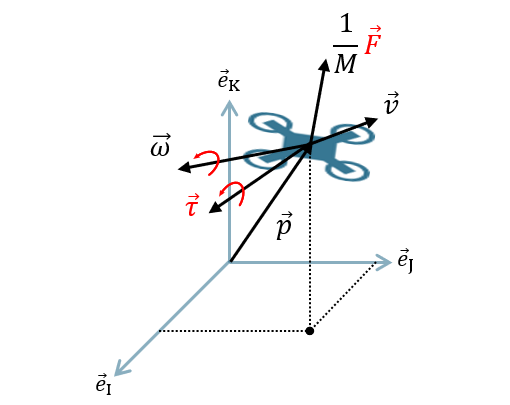
\includegraphics[width=0.8\textwidth]{ch2_drone_diagIJK}
%  \caption{Quad-Rotor's state vector diagram}
%  \label{fig:drone_diag}
%\end{figure}

\subsection{Defender-Attacker Reachability}
\label{ssec:area-defense}

%The scenario in study is a reach-avoid game between a defender drone and an attacker drone. The attacker's goal is to reach a critical area, and it may take any feasible trajectory that accomplishes this goal in reasonable time. The defender's goal is to reach the attacker before it reaches the critical area, despite the exact attacker trajectory not being known ahead of time. The challenge lies in ensuring that the set of possible defender trajectories fully intersects with the set of attacker trajectories at some moment in the future, thus ensuring the defender reaches the attacker and guaranteeing area defense.

The defender is a dynamic system $\dot{\xD} = f(\xD,\uD)$ with a bounded control input $\uD$, and the set that is guaranteed to contain all possible states for $\uD \in \mathcal{U}$ at a future time $k$ is called the defender reachable set and is denoted by $\ED_k$. An accurate but overly conservative $\ED_k$ for example, is $\ED_k = \mathbb{R}^n$. Ideally, $\ED_k$ is as accurate to the system's dynamics as possible, while remaining computationally efficient. The set containing all feasible trajectories from the current time $k=0$ to the prediction horizon $k=N$ is called the Defender Reachability Cone (DRC), denoted by $\RD$, and is considered to be the set of consecutive reachable sets in that time frame, that is, $\RD = \{\ED_k\}, \quad k=[0:N]$. The Attacker Reachability Cone (ARC) and reachable sets are denoted as $\RA = \{\EA_k\}, \quad k=[0:N]$. The defender can reach the attacker at any point in the future if the following holds:
\begin{equation}
    \exists \ED_i \in  \RD : \ED_i \cap \EA_i \supseteq \EA_i, \EA_i \in \RA, 0 \le i\le N.
    \label{eq:reach-condition}
\end{equation}
Intuitively, this means that if the intersection between the defender and attacker reachable sets ($\ED_i \cap \EA_i$) is a superset of the attacker reachable set ($\supseteq \EA_i$) at some moment in the future ($i$), then the defender can reach all positions the attacker can reach, as long as $\ED$ is an inner approximation and $\EA$ is an over-approximation. 
%Intuitively, this means that if there is a defender reachable set that fully intersects an attacker reachable set at some moment in the future, then interception is assured and area defense is guaranteed.

\subsection{Parametric Reachable Sets}
\label{sec:parametric-reachable-set}
Traditionally, reachable sets for linear dynamic systems are  approximated using CCGs~\cite{RegoF}~\cite{SilvestreD1}. However, CCGs tend to be computationally expensive and using them with non-linear systems requires linearizations of the system dynamics. Therefore the parametric reachable set via controlled dynamical embeddings is better suited for this work, as it doesn't require linearizing the model.

The parametric reachable set, referred to as a parametope~\cite{harapanahalli2025parametric}, is defined as

%To devise a computationally efficient reachable set representation of a quad-rotor drone, some background on parametric reachable sets is necessary. Here the reachable set is a dynamic parametric ellipsoid, referred to as a parametope~\cite{harapanahalli2025parametric}, and it is represented as
\begin{equation}
    ((\mathring{\xD}, \alphaD, \yD))_{\varepsilon} := \{ \xD \in \mathbb{R}^n : \ellip{\mathring{\xD}}{(\alphaD^T \cdot \alphaD)^{-1}} \le \yD \},
\end{equation}
where $\mathring{\xD}$ is the center, $\alphaD$ the parameter matrix and $\yD$ is the squared radius, and $\ellip{\vm{q}}{\vm{Q}}$ the function for an ellipsoid with center $\vm{q}$ and shape matrix $\vm{Q}$, given by
\begin{equation}
    \ellip{\vm{q}}{\vm{Q}} = (\vm{x}-\vm{q})^T \vm{Q}^{-1}(\vm{x}-\vm{q}).
\end{equation}
The parametope is propagated via the controlled dynamic embedding system
\begin{equation}
    \dot{\mathring{\xD}} = f(\mathring{\xD}, \mathring{\uD}), \quad \dot{\alphaD} = U(\mathring{\xD}, \alphaD, \yD), \quad \dot{\yD} = E(\mathring{\xD}, \alphaD, \yD),
\end{equation}
where the parameter dynamics function is defined as
\begin{equation}
    U = -\alphaD \text{Df}(\mathring{\xD}),
\end{equation}
where $\text{Df}$ is the jacobian, and the radius dynamics function is defined as
\begin{equation}
    E = c \cdot \yD,
\end{equation}
$c$ being an expansion coefficient. In~\cite{harapanahalli2025parametric}, $c$ is computed using the Interval Mixed Jacobian (IMJ) of the system which, in turn, is given by the natural inclusion function matrix of the system's jacobian, obtained through Interval Analysis (IA)~\cite{intervalAnalysis}. Tools such as~\cite{immrax} can efficiently build the smallest IMJ~\cite{mixed_jacobian_matrix}, however implementation of these tools lays outside the scope of this work. 

It is noted that in systems with partly decoupled dynamics, like the quad-rotor UAV which has decoupled altitude and attitude dynamics, the dynamic components most sensitive to disturbances will define the bounds of the IMJ, and the actual bounds of the less sensitive components are lost. This is noted with the quad-rotor UAV embeddings system, where the relevant spatial dynamics are overshadowed by the attitude dynamics.

The following scaling method is therefore proposed to compute $c$, using only the positional dynamics of the drone, and it is given by
\begin{equation}
    c(k) = \left(\frac{||\vm{p}_{\text{max}}(k)-\vm{p}(k)||}{\sqrt{\yD(k-1)}}-1 \right)/T_s,
\end{equation}
where which $\vm{p}$ is the translational component of the drone's state, $\vm{p}_{\text{max}}$ the furthest possible trajectory in the next time-step, and $T_s$ the sampling period of the simulation.

\section{Defense Controller Formulation}
\label{sec:defense-controller-formulation}

With the defense conditions defined in~\eqref{eq:reach-condition}, and the DRC and ARC defined as sets of dynamically evolving parametopes, the proposed defense control solution can be devised.  

Firstly, some notions of ellipsoidal calculus and similarity must be introduced. Consider that the spatial ellipsoid of $\ED$ is denoted by $\ED^3$ and it is given by the intersection between $\ED$ and the $\mathbb{R}^3$ hyperplane~\cite{ellipsoidal_calculus}, this is
\begin{equation}
    \ED^3 = \ED \cap \mathbb{R}^3,
\end{equation}
and the same applies for $\EA^3$. Computing the intersection of ellipsoids invariably requires the solution of an optimization problem~\cite{yousefi2018novel_ellip_intersection}~\cite{ros2002ellipsoidal} for each prediction step, at each simulation step, which is computationally untenable. 

In lieu of ellipsoid intersection, the KLD is used to quantify ellipsoid similarity. The KLD is traditionally used as a measure of similarity between two gaussian distributions, each described by a positive-definite symmetric covariance matrices, and it is a smooth, always positive, scalar-valued operation that tends to zero when the distributions are identical~\cite{duchi2007derivations}. Furthermore, the KLD is asymmetric~\cite{DKLvisual}. These characteristics make it a good candidate to quantify similarity between ellipsoids. The KLD from $\Omega_1$ to $\Omega_2$ with centers $\vm{q}_1$, $\vm{q}_2$ and shape matrices $\vm{Q}_1$, $\vm{Q}_2$ respectively, and dimensions $n \times n$, has the function notation \KLD{.}{.} and is given by
\begin{align}
    \KLD{\Omega_1}{\Omega_2} = &\frac{1}{2} ( \mathtt{tr}(\vm{Q}_2^{-1} \vm{Q}_2) + (\vm{q}_2-\vm{q}_1)^T \vm{Q}_2^{-1} (\vm{q}_2-\vm{q}_1) \nonumber\\
    &- n + \ln \left( \frac{\det \vm{Q}_2}{\det \vm{Q}_1} \right) ).
\end{align}
The array of pairwise KLD operations between elements of $\RA$ and $\RD$ is denoted by $\bKLD{\RA}{\RD}$ such that
\begin{equation}
    \bKLD{\RA}{\RD} := [\KLD{\EA_k}{\ED_k}], \quad k=[0:N].
\end{equation}

The \verb|min| operator is not continuous, which makes it unsuitable for optimization problems~\cite{GilpinSTLlse}. The LSE function, denoted by \LSE{.}, poses a smooth under-approximation of the \verb|min| operator as seen in~\cite{LindemannCBFlse}.

Before moving on, a disclaimer is called for. Recalling~\eqref{eq:reach-condition}, the defender can reach all positions the attacker can reach at some moment $i$, if $\ED_i \cap \EA_i \supseteq \EA_i$ and $\ED_i$ is an inner approximation. Since the defender set is defined as a parametope, which is an over-approximation, only the first part of the condition may hold, which does not guarantee interception. However, it is considered that the larger the volume of $\ED_i^3 \cap \EA_i^3$, the more likely the defender is to intercept the attacker. With this approach in mind, the proposed control architecture is presented in the following section.

\subsection{Control Architecture}
The controller receives as input the current defender state $\xD$ and current DRC $\RD$, as well as the current attacker state $\xA$, reachable set parameter matrix $\alphaA$ and reachable set radius $\yA$. Knowing the attacker model, $\RA^3$ can be pre-computed in full before being passed as parameters to the numerical solver, to ease the computational burden.
Computing the full $\RD$ trajectory online is impractical however, as the objective function becomes far too complex for the solver to handle, being composed of dozens of thousands of sub-functions. For this reason, a reduced ellipsoid $\ED'$ is used in the defender's case, where 
\begin{align}
    &\ED' = \varepsilon (\pD, \vm{W}),\\
    &\vm{W}= \dcmD \cdot \left(\yD \begin{bmatrix}
        1 & 0 & 0 \\
        0 & 1 & 0 \\
        0 & 0 & 0.1
    \end{bmatrix}
    \right) \cdot \dcmD^T,
\end{align}
The set of all 3-dimensional reduced defender ellipsoids for predicted time-steps is denoted $\RD'$.

In following, the components of the NMPC objective function components are defined and briefly explained, before joining them together.
Consider the minimum KLD from $\EA_k^3$ to $\ED_k'$, $k=[0:N]$, to be
\begin{equation}
    d_{AD} = \LSE{\bKLD{\RA^3}{\RD'}},
\end{equation}
and the symmetric counterpart,
\begin{equation}
    d_{DA} = \LSE{\bKLD{\RD'}{\RA^3}},
\end{equation}
and assume that both values correspond to the pair of concurrent ellipsoids $\ED_i'$ and $\EA_i^3$ closest to each other. In the final stage of approach, when there is overlap between $\RD'$ and $\RA^3$, in order for the reach condition defined in~\eqref{eq:reach-condition} to be satisfied, then the inequality $d_{AD} \le d_{DA}$ must be verified. Thus, the system should evolve such that $d_{AD}$ decreases faster than $d_{DA}$, which is enforced by minimizing $d_{AD}$ and at the same time maximizing $d_{DA}$ in the objective function.

The relevant minimum KLD is the one between the pair of concurrent ellipsoids which are nearest. This is enforced by introducing the term $e$ in the objective function, which is the minimum of the set of ellipsoid center error norms, denoted as 
\begin{equation}
    e = \LSE{[||\pD_k-\pA_k||_2]}, \quad k=[0:N],
\end{equation}
where $\pA_k$ is the attacker positional variables.

\begin{figure}[htbp]
    \centering
    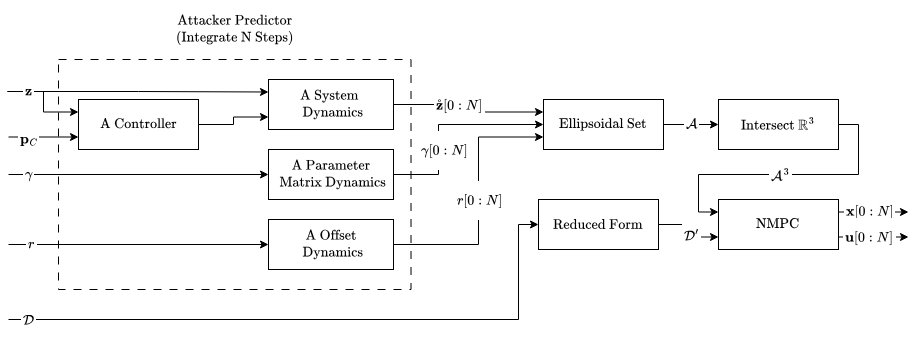
\includegraphics[width=0.9\columnwidth]{NMPCdiag}
    \caption[Diagram of defense controller]{Data flow diagram of defense-centric controller.}
    \label{fig:NMPC_diag}
\end{figure}

This all comes together in the optimization problem
\begin{align}
    \min_{X,U} &\quad  e Q_e + d_{AD}Q_{AD} - d_{DA}Q_{DA} + \sum_{k = 1}^{N} ||\uD_k||^2_2 R \nonumber\\
    s.t.: &\quad \xD_0 = \vm{x0} \nonumber\\
    &\quad \xD_{k+1} = f(\xD_k, \uD_{k}), \nonumber\\
    &\quad \xD \in \mathcal{X}  \nonumber\\
    &\quad \uD \in \mathcal{U}
\end{align}

where $N$ is the prediction horizon, $f(.,.)$ is the quad-rotor's dynamics function, and $Q_e$, $Q_{AD}$, $Q_{DA}$ and R are the weight matrices.
The optimization variables are $X = [\xD_k]$ and $U = [\uD_{k}]$, and the parameters are $\vm{x0}$, $\yD_k$ and $\RA^3$. The data flow diagram for the defender controller is shown in Figure~\ref{fig:NMPC_diag}.

\subsection{Safe Reachability Cone}
\label{sec:safe-reachability-cone}
The Safe Reachability Cone (SRC) is the set of trajectories predicted to be denied from the attacker, and is a useful tool to validate and visualize a defensive trajectory. It is represented as
\begin{equation}
    \RS = [\ES_k], \quad i\le k \le N,
\end{equation}
where $\ES_k$ is the safe reachability set at time-step $k$, and $i$ is the time-step the defender is predicted to reach the attacker. $\ES$ is a parametope defined as
\begin{equation}
    \ES = ((\mathring{\vm{x}}_{S}, \alphaA, \yA))_{\varepsilon},
\end{equation}
propagated via the controlled dynamic embedding system
\begin{equation}
    \dot{\mathring{\vm{x}}}_{S} = q(\mathring{\xA})+\vm{x}_{o}, \quad \dot{\alphaA} = U(\mathring{\xA}, \alphaA, \yA), \quad \dot{\yA} = E(\mathring{\xA}, \alphaA, \yA),
\end{equation}
where $q(.)$ is the attacker dynamics, $\xA$ the attacker state vector, $\alphaA$ the attacker parameter matrix with initial value set at $\alphaD_i$, and $\yA$ is the attacker squared radius with initial value $\yD_i$. $\vm{x}_o$ is an offset which aligns the central predicted attacker trajectory with $\ED_i$. The SRC in a simplified reach-avoid scenario is illustrated in Figure~\ref{fig:safeguarded_space_sim}.
\begin{figure}[htbp]
    \centering
    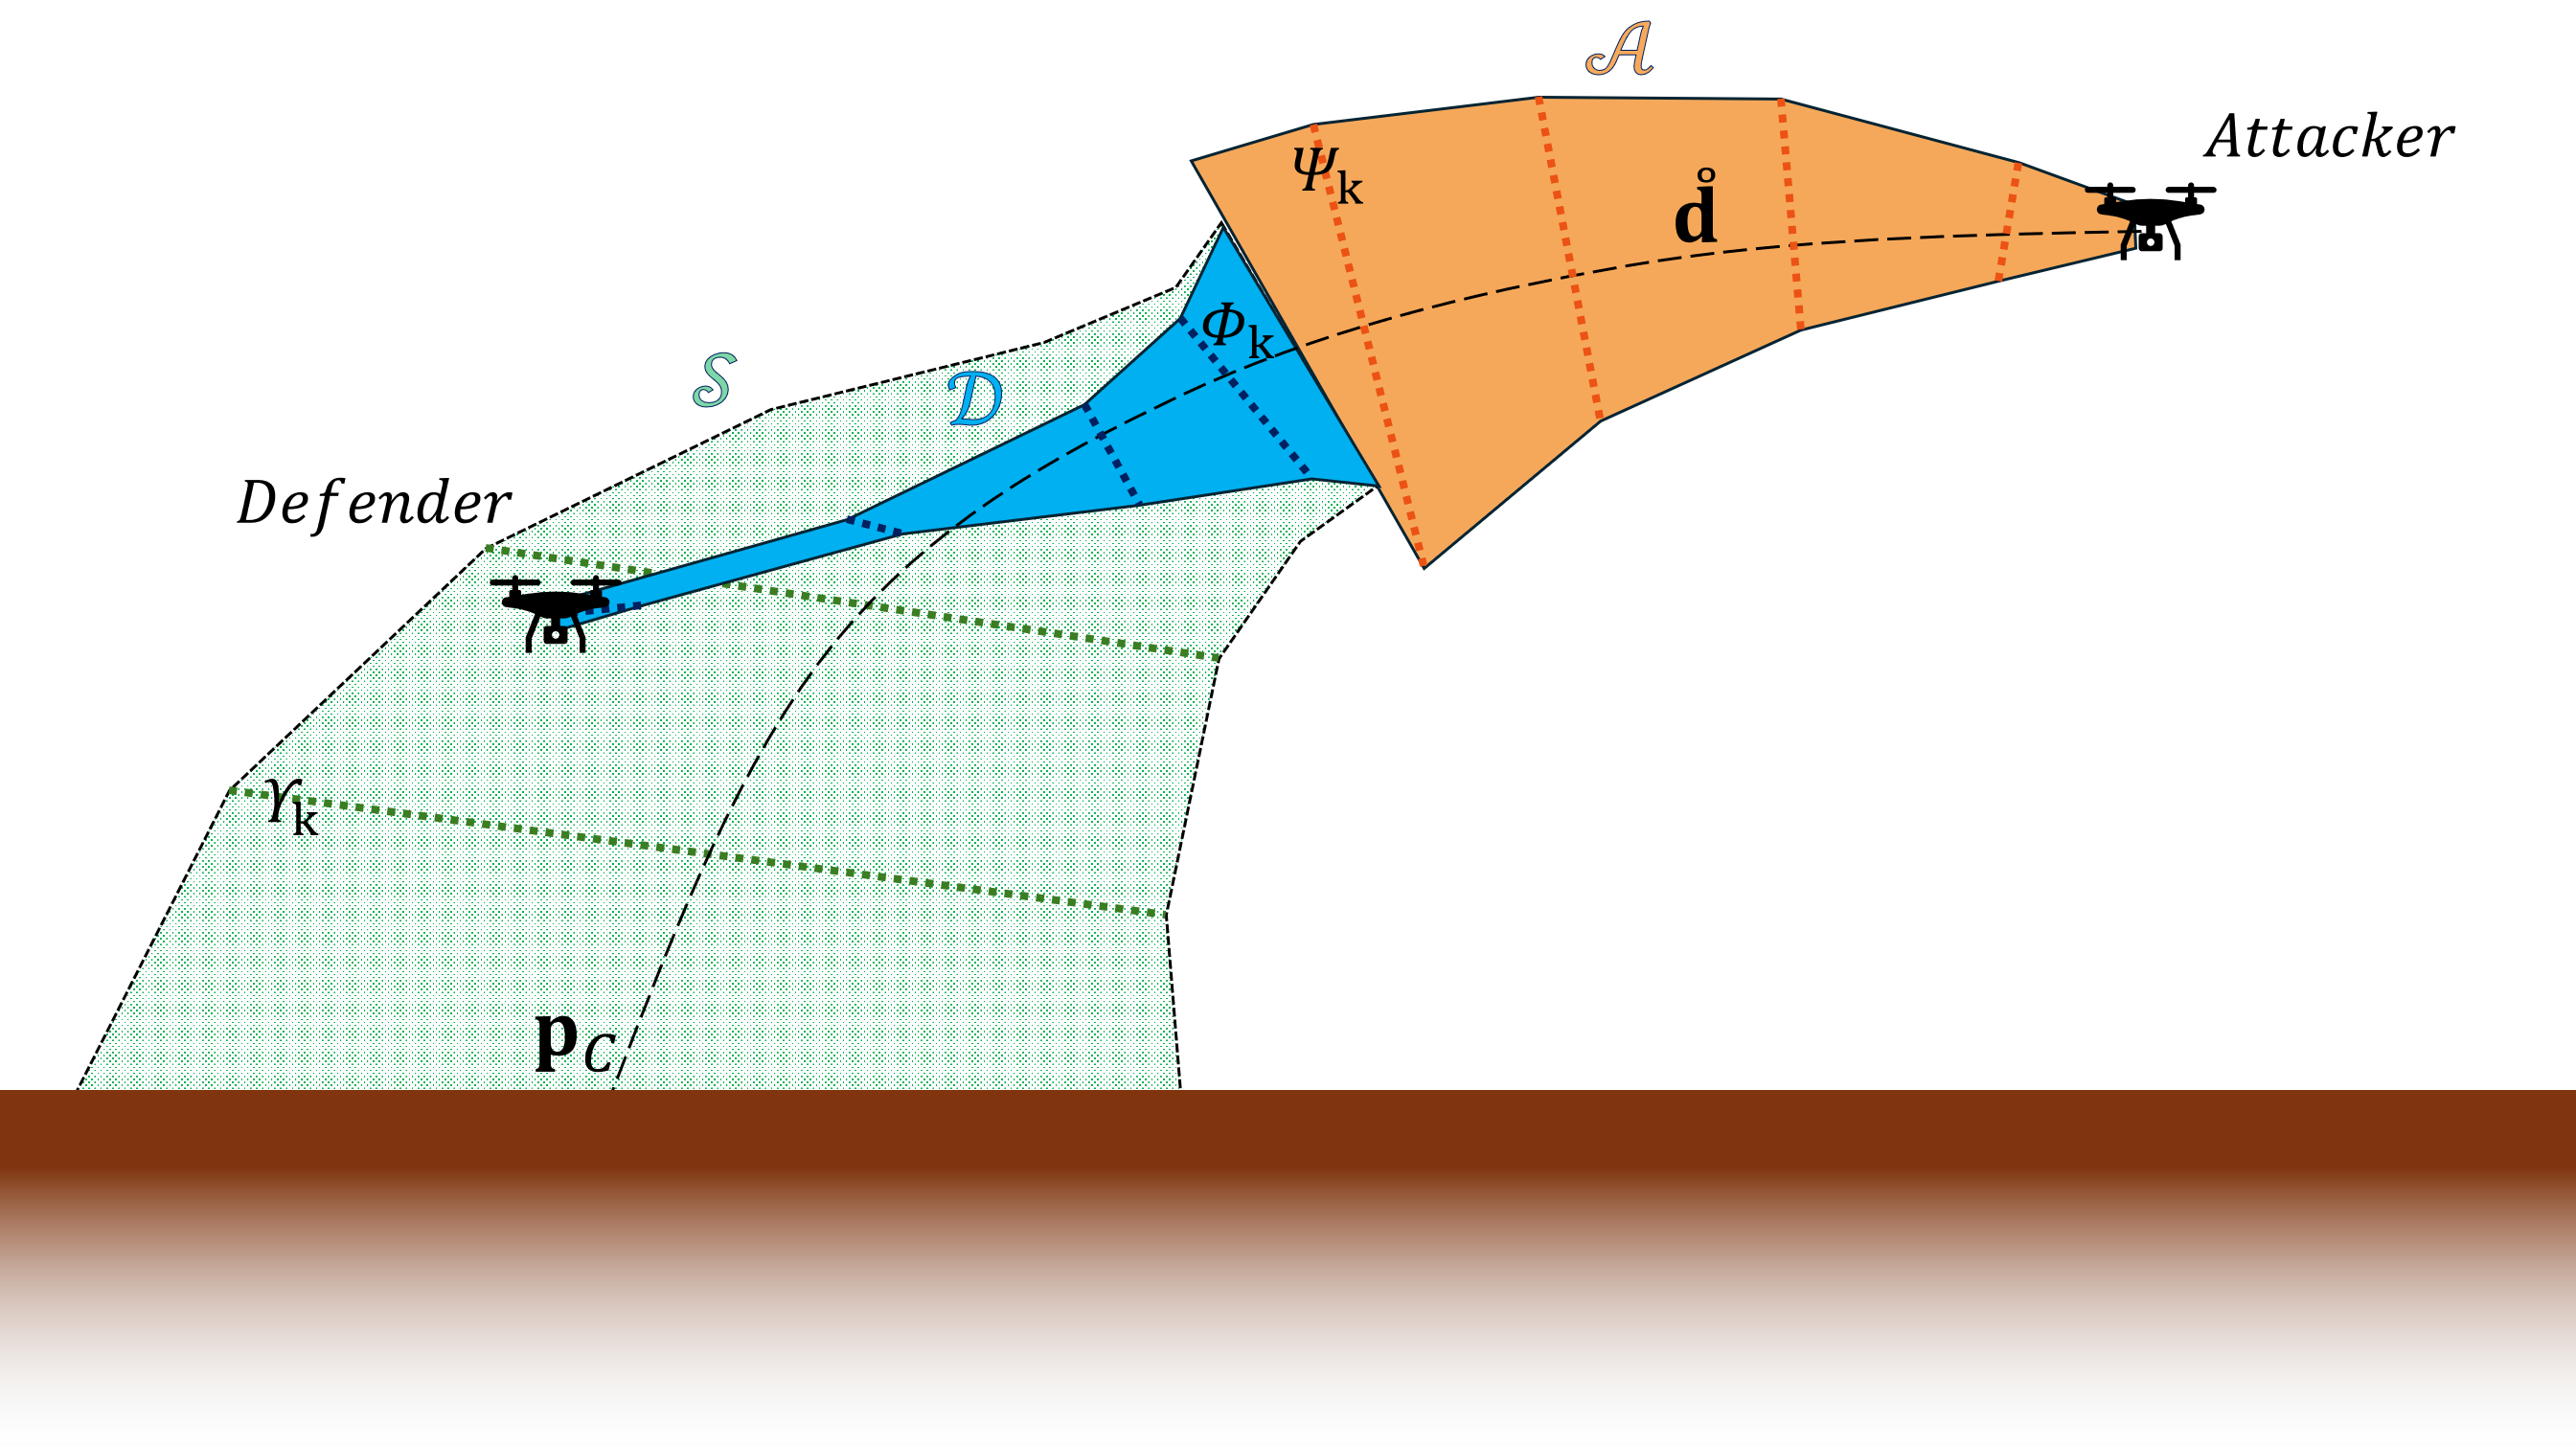
\includegraphics[width=0.9\columnwidth]{safeguardedAreaFig}
    
    \caption[Illustration of safeguarded area]{Illustration of safeguarded area: 2-dimensional simplification. For $k=[0:N]$, $RD = [\ED_k]$ is the DRC, $\RA = [\EA_k]$ is the ARC, and $\RS = [\ES_k]$ is the SRC.}
    \label{fig:safeguarded_space_sim}
\end{figure}

\section{Simulations and Discussion}
\label{sec:simulations-and-discussion}

\subsection{Reachable Set Validation}
A simulation of a quad-rotor model moving from an initial hovering position to another hovering position was run with MATLAB~\cite{MATLAB} to verify the accuracy of the reachable set, outlined in Section~\ref{sec:parametric-reachable-set}, when compared to potential trajectories. Predicted state trajectories are computed from the current moment to the prediction horizon by fixing the drone's torque input $[\uD_2;\uD_3;\uD_4]$ as combinations of the maximum, minimum, and middle values, and the $\uD_1$ input at its minimum or maximum. The drone's physical parameters are in Table~\ref{tab:quadrotor_parameters}, and the input bounds are in Table~\ref{tab:quadrotor_variable_bounds}.

In both the following figures, the $k_{sim}$ axis indicates the real-time time-steps, and the $k_{pred}$ axis indicates the predicted time-steps. Figure~\ref{fig:reach-set-median-error} shows the median distance between the reachable set surface and the trajectories it contains at the respective time-steps, where positive values indicate the trajectory is contained in the set, and negative values that it's outside. Figure~\ref{fig:reach-set-volume-error} shows the volume difference between the reachable set and the convex hull formed by the trajectories.

\begin{figure}[htbp]
    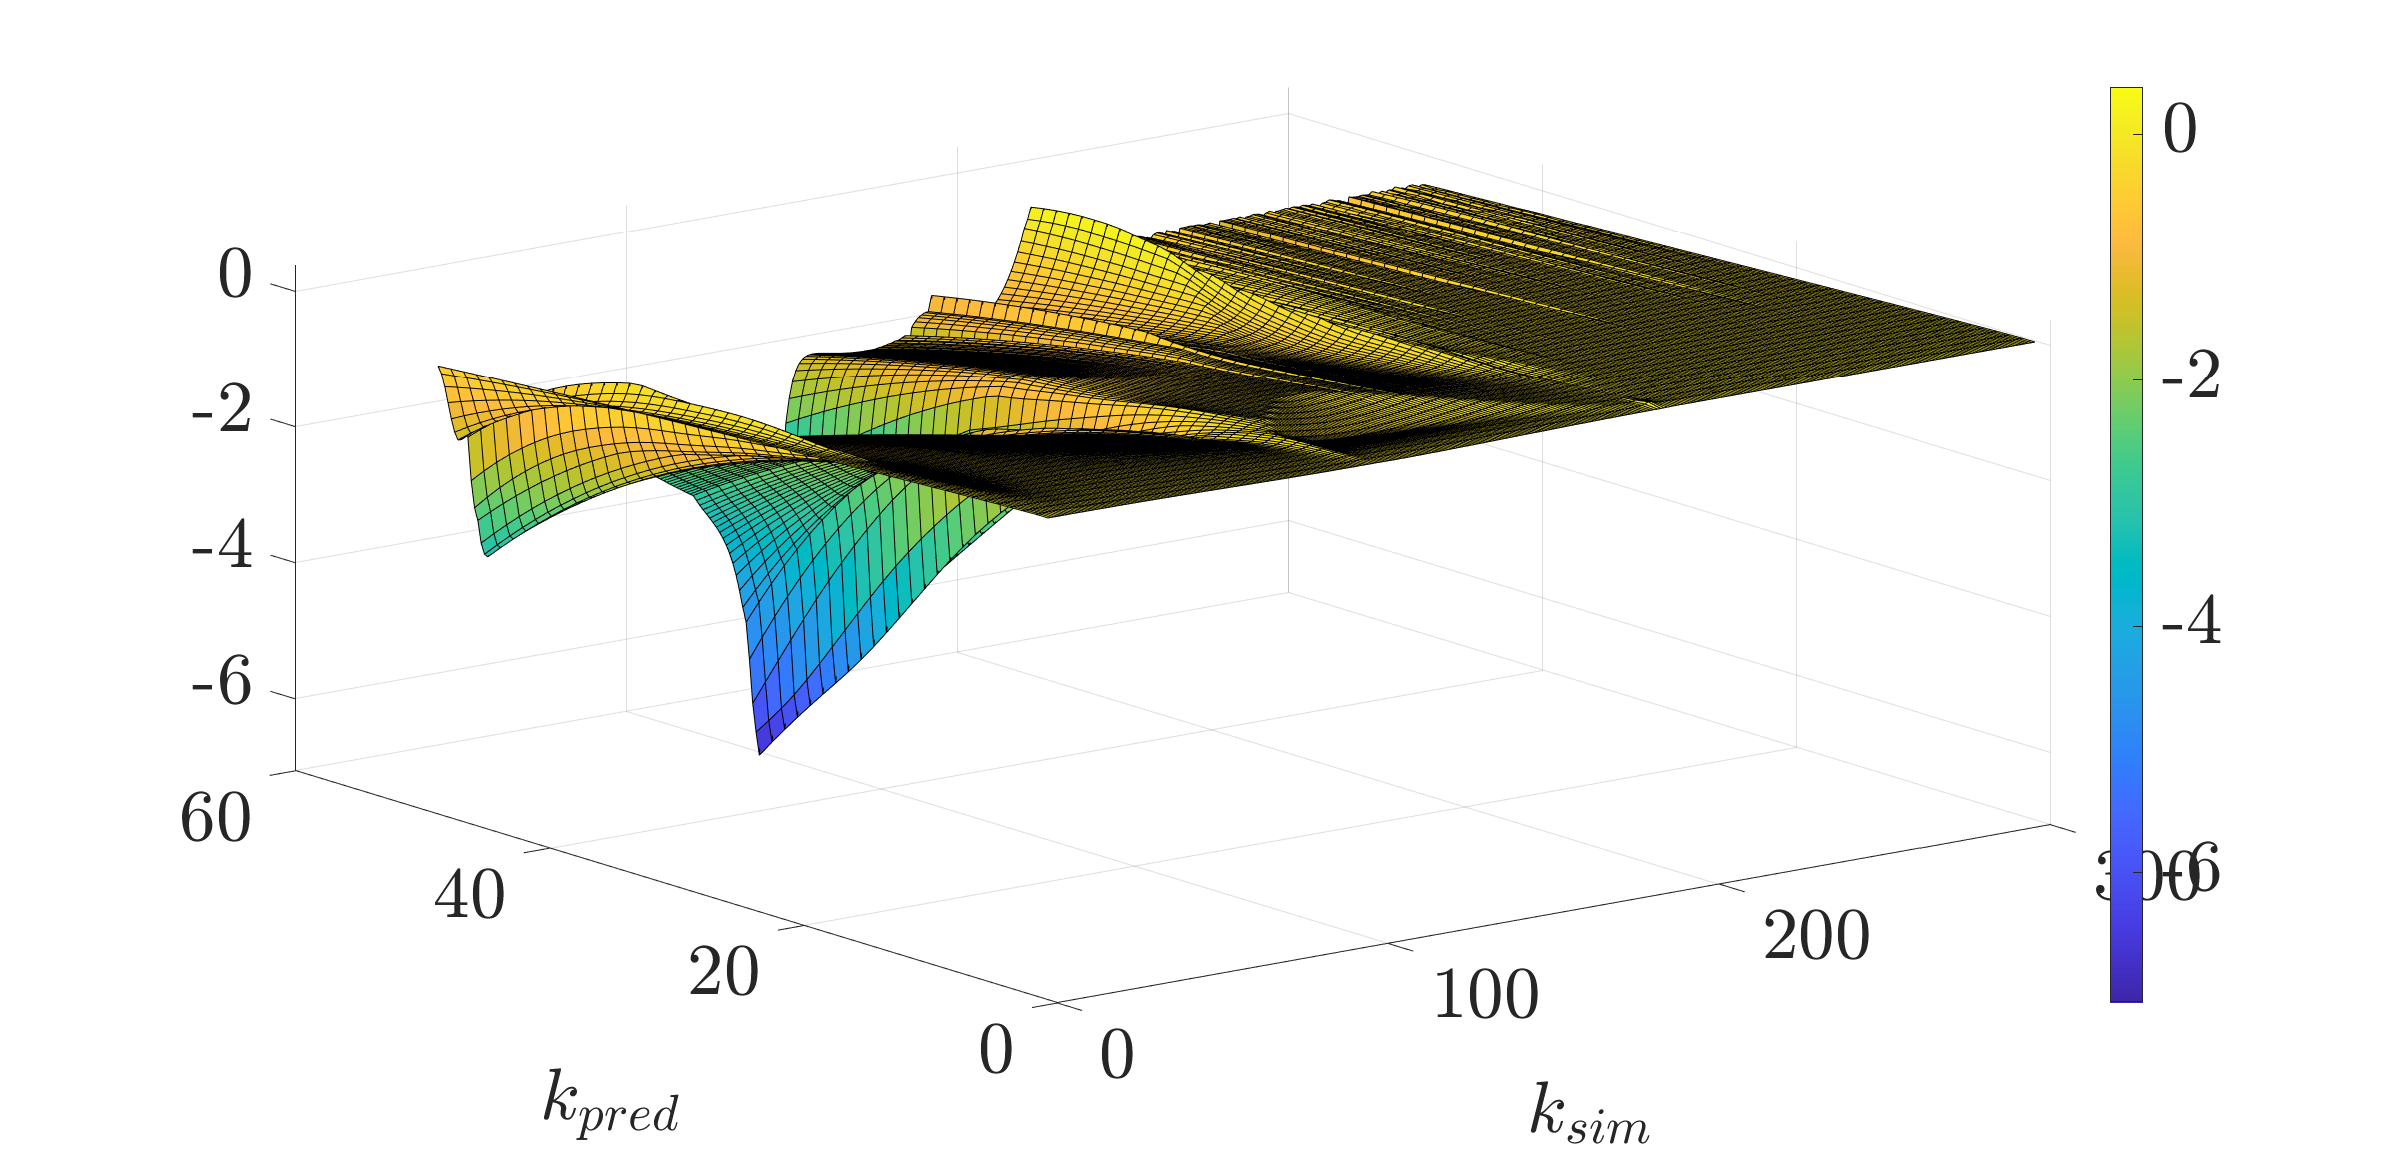
\includegraphics[width=0.9\columnwidth]{monteCarloME_N50}
    \caption[short]{Median distance between reachable set surface and potential predicted trajectories.}
    \label{fig:reach-set-median-error}
\end{figure}

\begin{figure}[htbp]
    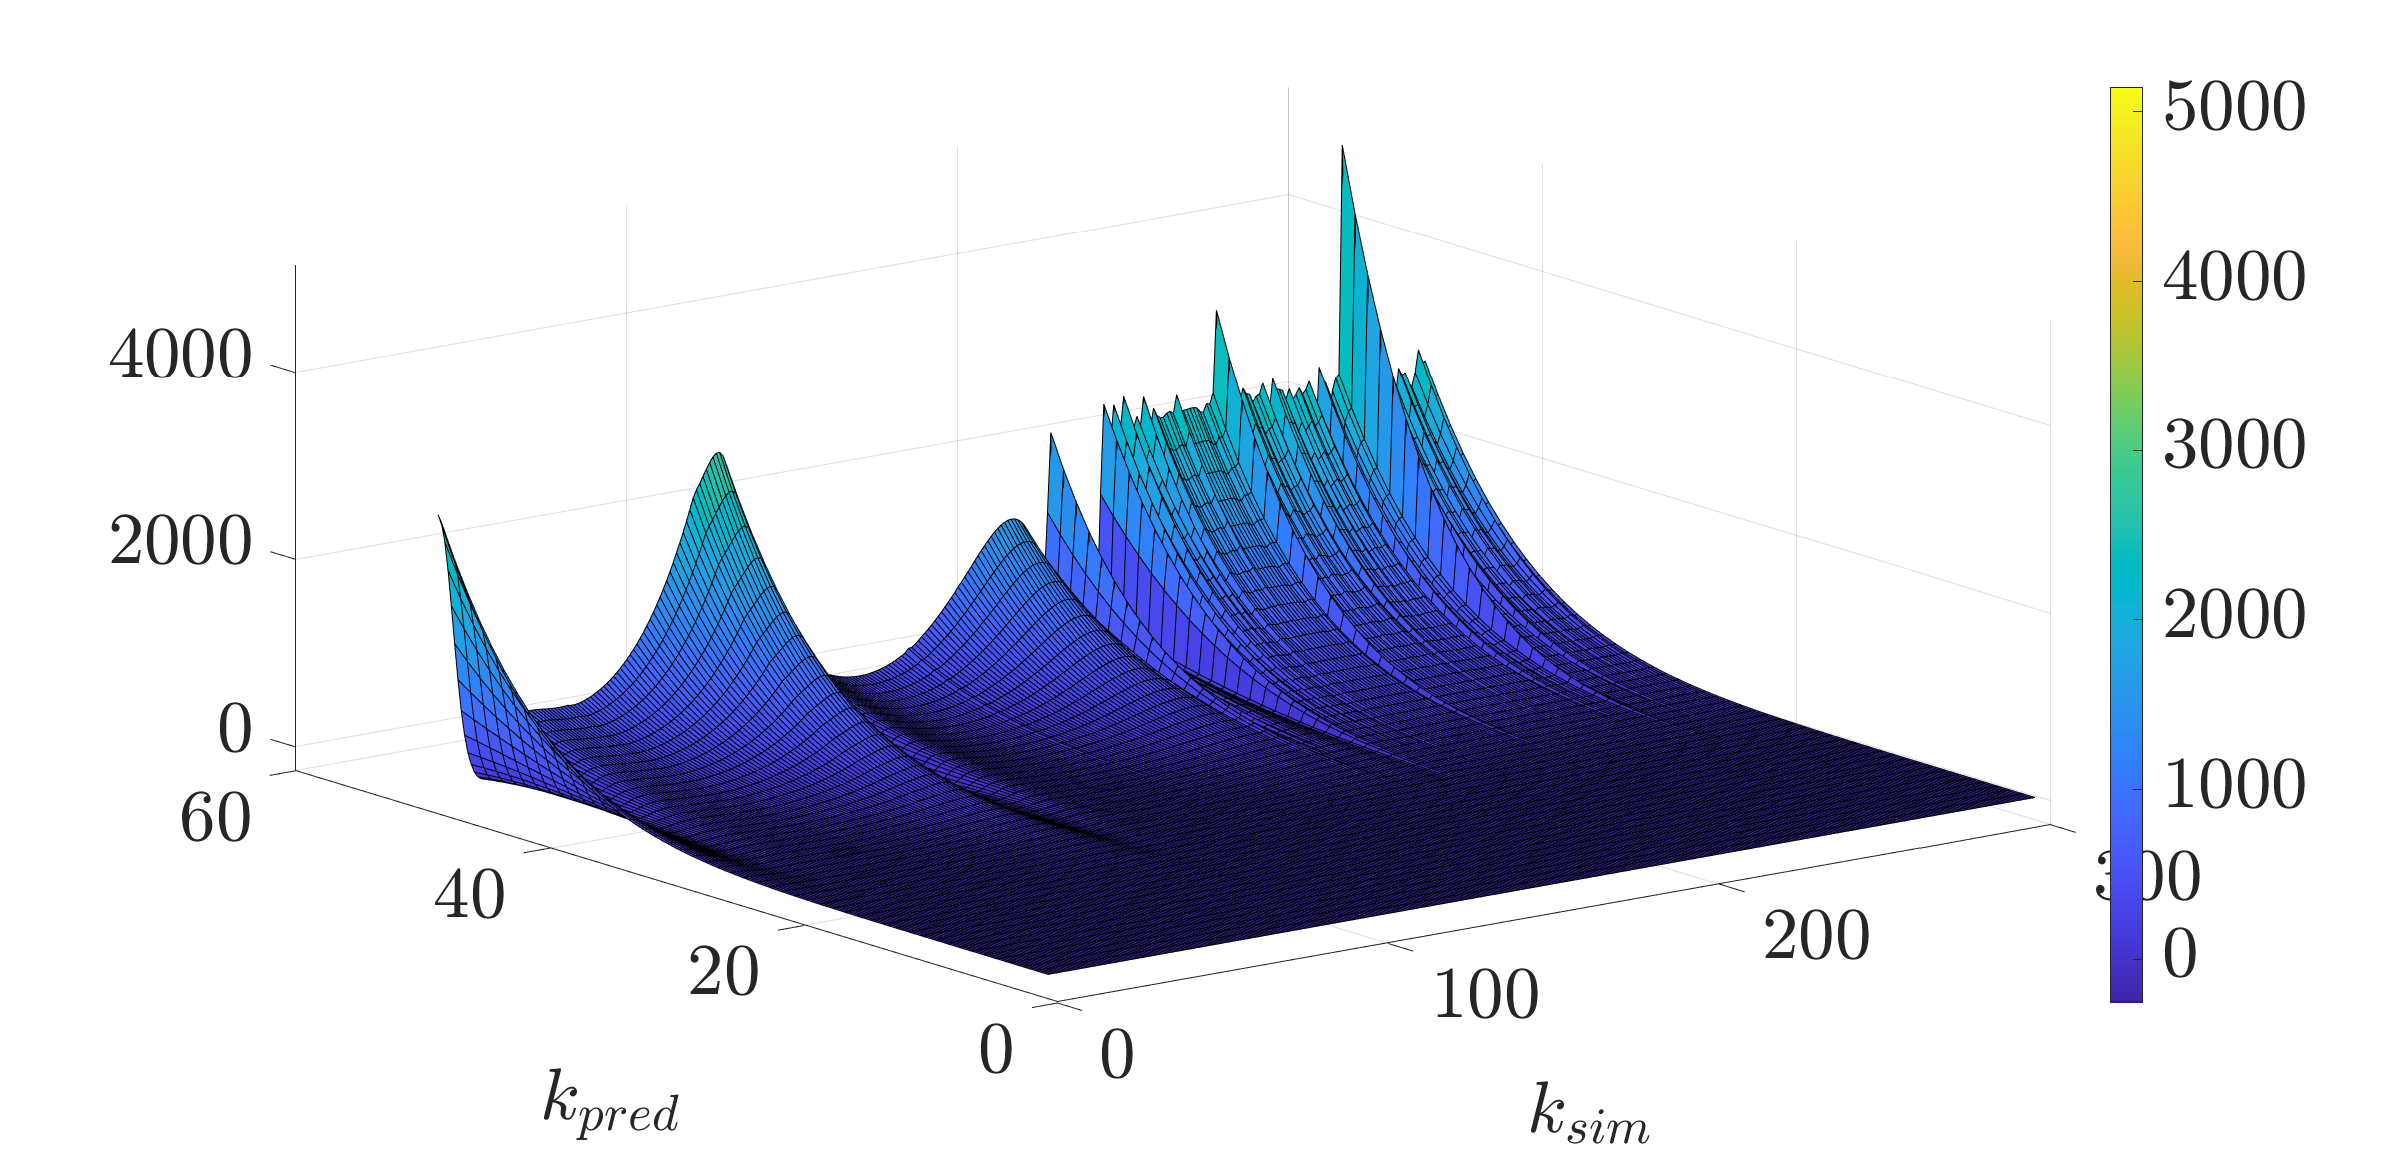
\includegraphics[width=0.9\columnwidth]{monteCarloVolE_N50}
    \caption[short]{Volume difference between reachable set and convex hull of trajectories.}
    \label{fig:reach-set-volume-error}
\end{figure}

\subsection{Two Drone Scenario}
A reach-avoid scenario is simulated with MATLAB~\cite{MATLAB}, in which the attacker drone moves toward the critical area, set at the origin, and has a polynomial trajectory planner in series with a Mellinger controller~\cite{Mellinger} as the control architecture. Furthermore, the attacker's trajectory is made unpredictable by repeatedly shifting the target waypoint by random amounts. The defender drone is initially hovering above the critical area. Both drones are quad-rotor UAVs, and their physical parameters are in Table~\ref{tab:quadrotor_parameters}, and their input bounds are in Table~\ref{tab:quadrotor_variable_bounds}.

\begin{table}[!t]
\renewcommand{\arraystretch}{1.3}
\caption{Quad-Rotor Parameters}
\label{tab:quadrotor_parameters}
\begin{center}
\begin{tabular}{cccclllllll}
\cline{1-4}
\multicolumn{1}{c|}{Parameter} & \multicolumn{1}{c|}{Description}             & \multicolumn{1}{c|}{Units}                     & Value                &  &  &  &  &  &  &  \\ \hhline{=|=|=|=~~~~~~~}
\multicolumn{1}{c|}{$M$}       & \multicolumn{1}{c|}{Total Mass}              & \multicolumn{1}{c|}{$\text{kg}$}               & $0.5$                &  &  &  &  &  &  &  \\ \cline{1-4}
\multicolumn{1}{c|}{$L$}       & \multicolumn{1}{c|}{Arm Length}              & \multicolumn{1}{c|}{$\text{m}$}                & $0.25$               &  &  &  &  &  &  &  \\ \cline{1-4}
\multicolumn{1}{c|}{$I_x$}     & \multicolumn{1}{c|}{Angular Momentum x axis} & \multicolumn{1}{c|}{$\text{J} \cdot \text{s}$} & $0.0196$             &  &  &  &  &  &  &  \\ \cline{1-4}
\multicolumn{1}{c|}{$I_y$}     & \multicolumn{1}{c|}{Angular Momentum y axis} & \multicolumn{1}{c|}{$\text{J} \cdot \text{s}$} & $0.0196$             &  &  &  &  &  &  &  \\ \cline{1-4}
\multicolumn{1}{c|}{$I_z$}     & \multicolumn{1}{c|}{Angular Momentum z axis} & \multicolumn{1}{c|}{$\text{J} \cdot \text{s}$} & $0.0264$             &  &  &  &  &  &  &  \\ \cline{1-4}
\multicolumn{1}{l}{}           & \multicolumn{1}{l}{}                         & \multicolumn{1}{l}{}                           & \multicolumn{1}{l}{} &  &  &  &  &  &  &  \\
\multicolumn{1}{l}{}           & \multicolumn{1}{l}{}                         & \multicolumn{1}{l}{}                           & \multicolumn{1}{l}{} &  &  &  &  &  &  &  \\
\multicolumn{1}{l}{}           & \multicolumn{1}{l}{}                         & \multicolumn{1}{l}{}                           & \multicolumn{1}{l}{} &  &  &  &  &  &  &  \\ 
\end{tabular}
\end{center}
\end{table}

\begin{table}[!t]
\renewcommand{\arraystretch}{1.3}
\caption{Quad-Rotor Input Bounds}
\label{tab:quadrotor_variable_bounds}
\centering
\begin{tabular}{cccclllllll}
\cline{1-4}
\multicolumn{1}{c|}{Variable} & \multicolumn{1}{c|}{Units}                           & \multicolumn{1}{c|}{Lower bound} & Upper bound          &  &  &  &  &  &  &  \\ \hhline{=|=|=|=~~~~~~~}
\multicolumn{1}{c|}{$u_1$}    & \multicolumn{1}{c|}{$N$}                             & \multicolumn{1}{c|}{$0.0001$}    & $50$                 &  &  &  &  &  &  &  \\ \cline{1-4}
\multicolumn{1}{c|}{$u_2$}    & \multicolumn{1}{c|}{$\text{rad}\cdot \text{s}^{-2}$} & \multicolumn{1}{c|}{$-2 \pi$}    & $2 \pi$              &  &  &  &  &  &  &  \\ \cline{1-4}
\multicolumn{1}{c|}{$u_3$}    & \multicolumn{1}{c|}{$\text{rad}\cdot \text{s}^{-2}$} & \multicolumn{1}{c|}{$-2 \pi$}    & $2 \pi$              &  &  &  &  &  &  &  \\ \cline{1-4}
\multicolumn{1}{c|}{$u_4$}    & \multicolumn{1}{c|}{$\text{rad}\cdot \text{s}^{-2}$} & \multicolumn{1}{c|}{$-2 \pi$}    & $2 \pi$              &  &  &  &  &  &  &  \\ \cline{1-4}
                              &                                                      &                                  &                      &  &  &  &  &  &  &  \\
\multicolumn{1}{l}{}          & \multicolumn{1}{l}{}                                 & \multicolumn{1}{l}{}             & \multicolumn{1}{l}{} &  &  &  &  &  &  &  \\
\multicolumn{1}{l}{}          & \multicolumn{1}{l}{}                                 & \multicolumn{1}{l}{}             & \multicolumn{1}{l}{} &  &  &  &  &  &  &  \\
\multicolumn{1}{l}{}          & \multicolumn{1}{l}{}                                 & \multicolumn{1}{l}{}             & \multicolumn{1}{l}{} &  &  &  &  &  &  & 
\end{tabular}
\end{table}

A series of images showing this simulation from the initial moment to the moment the defender reaches the attacker are in Figure~\ref{fig:DvAfig_N50_s_unp}, where $\RD$ are the blue ellipsoids and $\RA$ are the orange ellipsoids. The simulation shows the defender speeding towards the attacker, then as $\RD$ and $\RA$ overlap the defender slows down as there is a $\ED_i$ which expands to contain the corresponding $\EA_i$. This can be seen as the defender positioning itself such that there is a moment it can reach any trajectory the attacker may take.

The defender's performance data is shown in Figure~\ref{fig:DvAerr_N50_s_unp}, where the top graph shows the norm of the distance between defender and attacker throughout the simulation, and the bottom graph shows the area of $\RA^3 \cap \mathcal{G}$ in blue, and $\RS^3 \cap \mathcal{G}$ in orange, denoted by $\Theta_A$ and $\Theta_S$ respectively, with $\mathcal{G}$ being the $\mathbb{R}^3$ ground plane. It can be seen that $\Theta_S$ fully overlaps $\Theta_A$ from approximately $t=0.1s$ to $t=0.3s$, which indicates that throughout this timeframe the defender is positioned such that it can reach all attacker trajectories.

%A: p0=(20,-20,5), vf=10*tf*(-1,1,0.5)/||(-1,1,0.5)||, af=10*(-1,1,0.5)/||(-1,1,0.5)||

\begin{figure}[htbp]
  \centering
    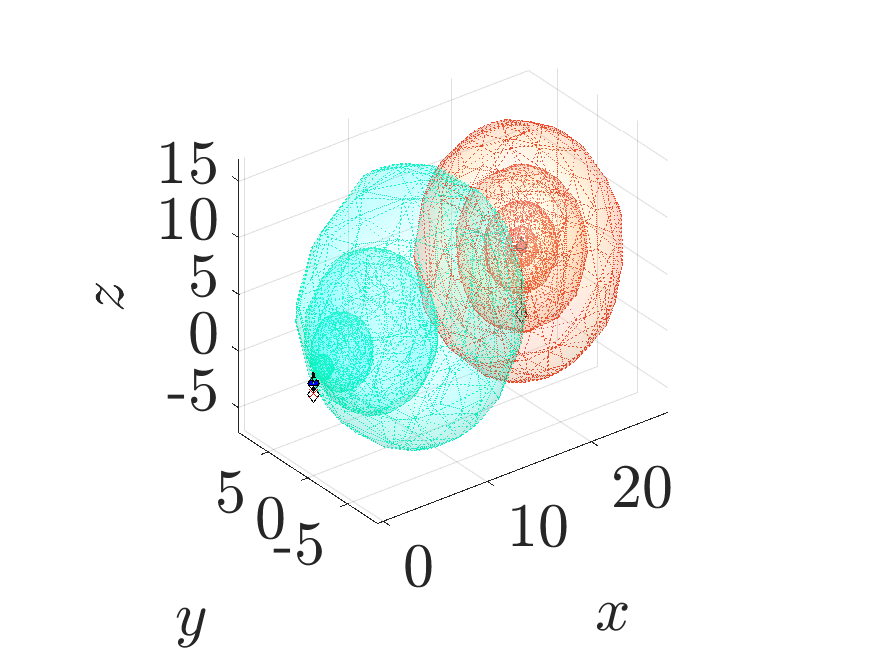
\includegraphics[width=0.45\columnwidth]{DvAfig_N50_s_unp1}
    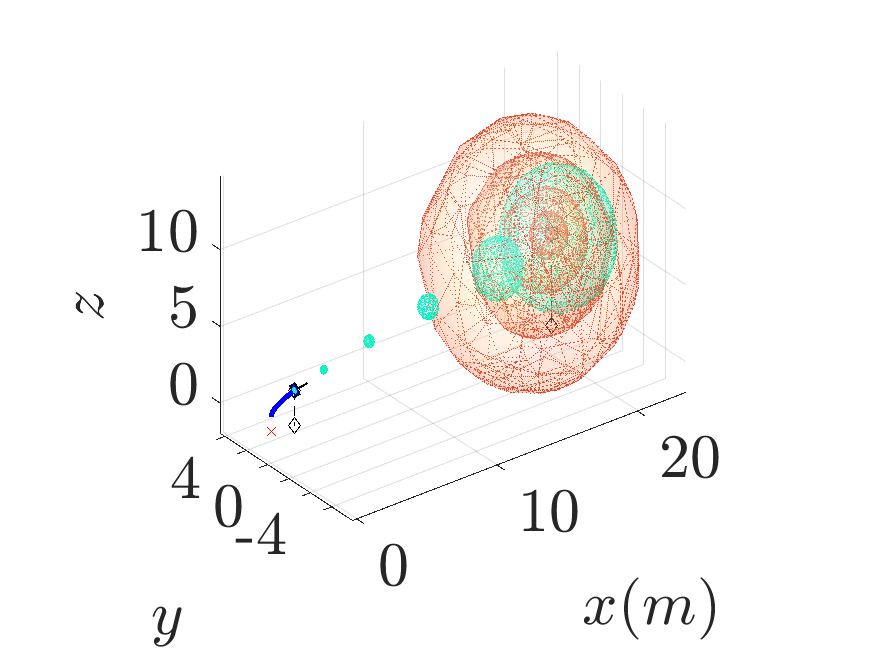
\includegraphics[width=0.45\columnwidth]{DvAfig_N50_s_unp2}\\
    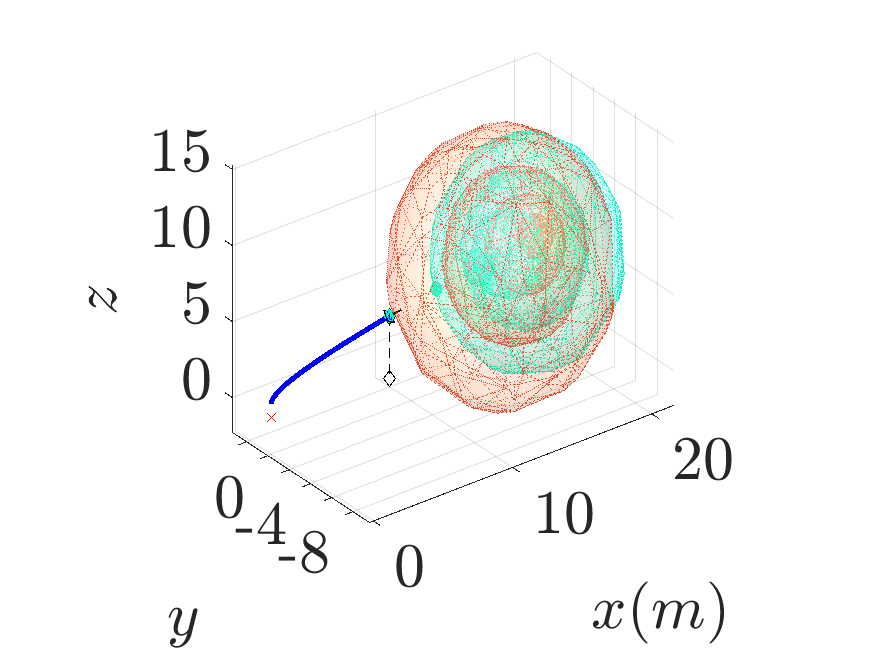
\includegraphics[width=0.45\columnwidth]{DvAfig_N50_s_unp3}
    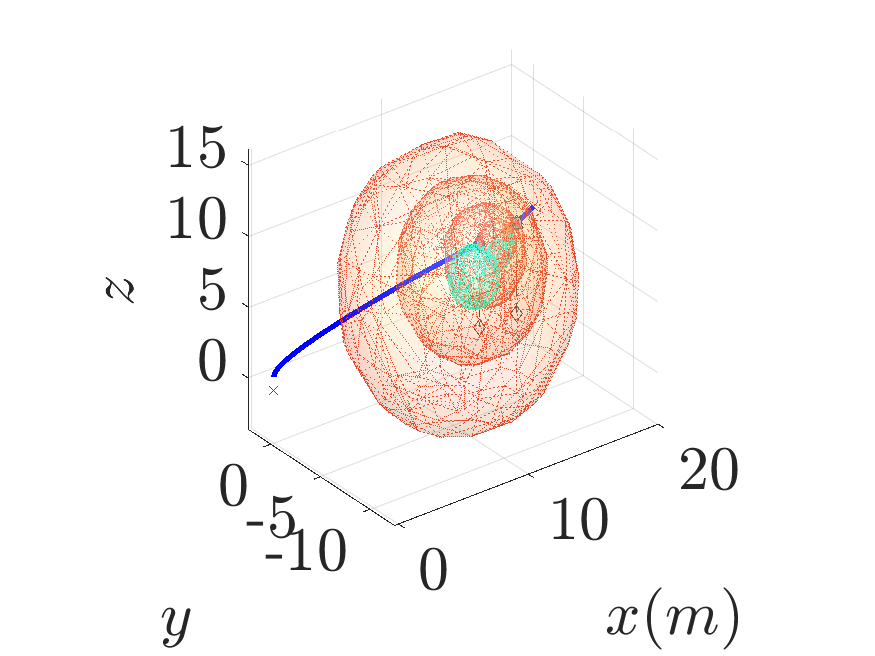
\includegraphics[width=0.45\columnwidth]{DvAfig_N50_s_unp4}\\
  \caption[Visualization of single D with defense controller vs. unpredictable A]{Visualization of single defender with defense-centric controller vs unpredictable attacker with Mellinger controller in defense scenario, N=50.}
  \label{fig:DvAfig_N50_s_unp}
\end{figure}
\begin{figure}[htbp]
  \centering
    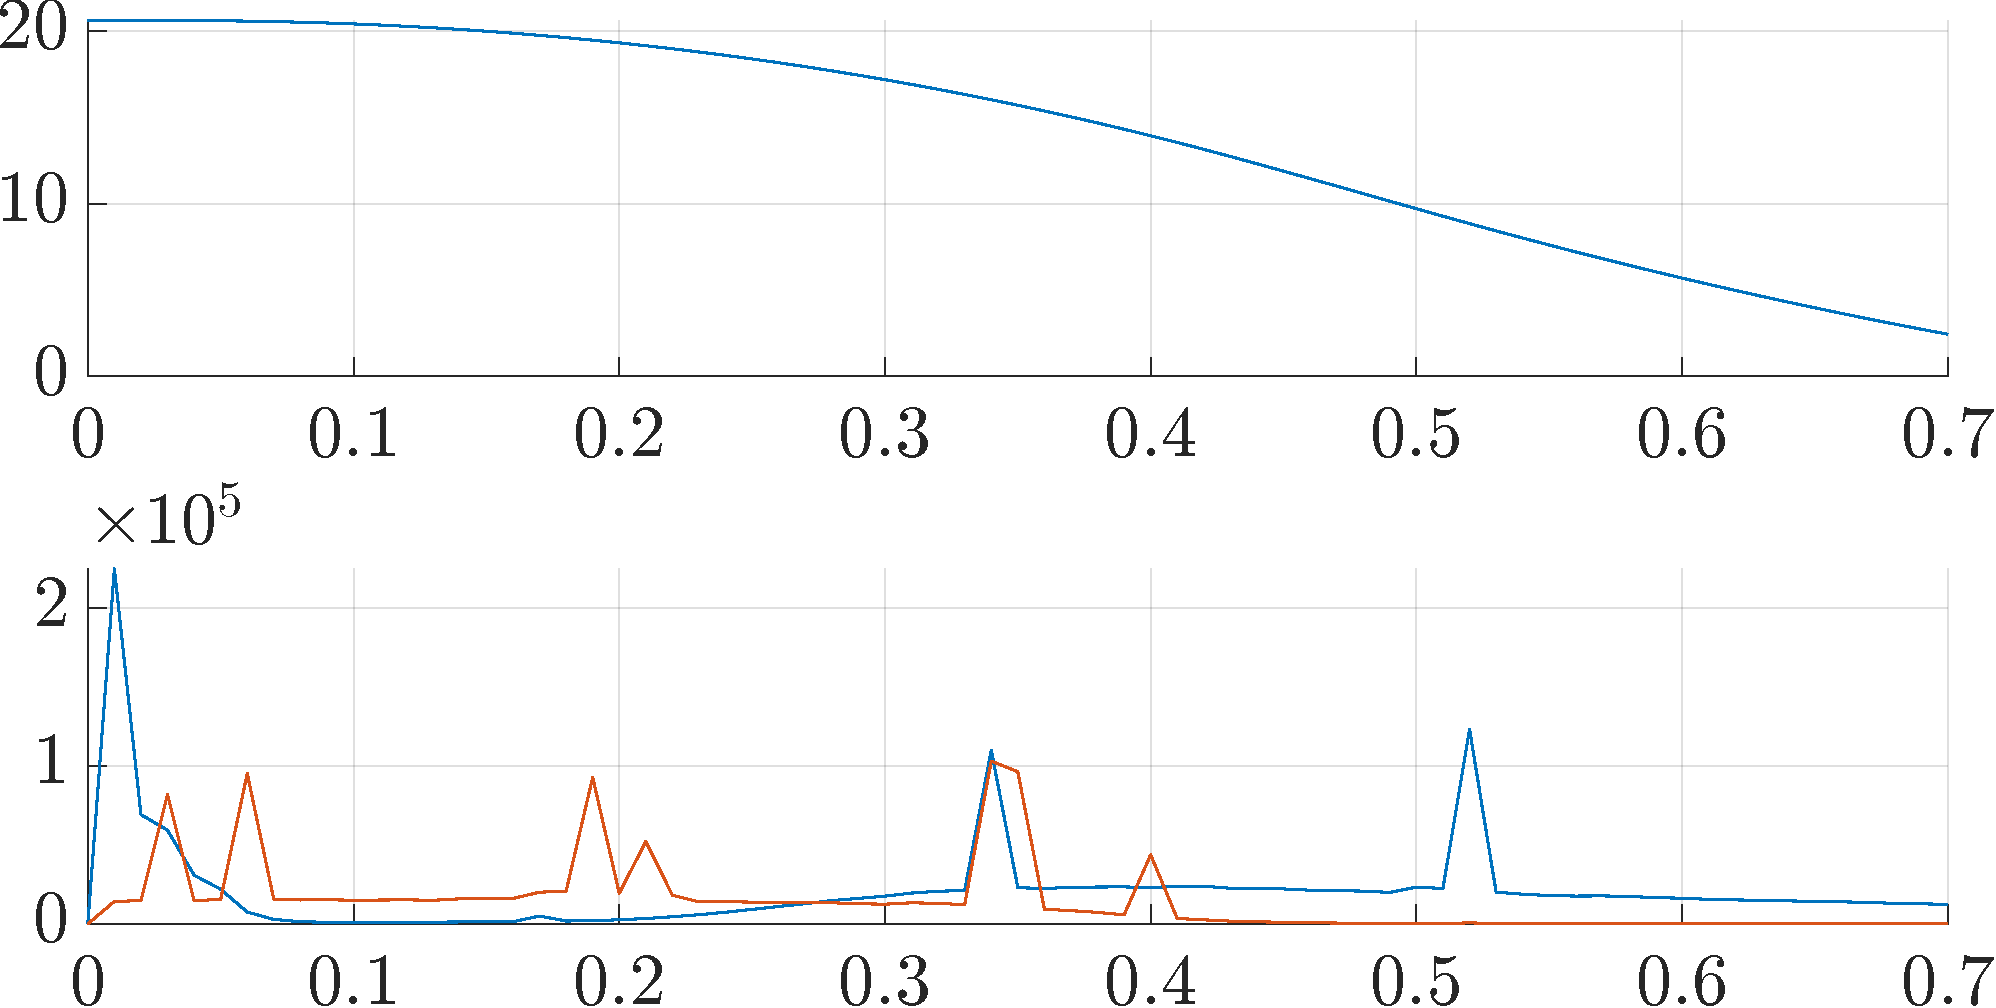
\includegraphics[width=0.9\columnwidth]{DvAerr_N50_s_unp}
  \caption[Performance analysis of defense controller in 1D vs. 1 unpredictable A scenario]{Performance analysis of  defense-centric controller in defense scenario with 1 defender and 1 unpredictable attacker.}
  \label{fig:DvAerr_N50_s_unp}
\end{figure}

\section{Conclusions and Further Work}
\label{sec:conclusions-and-further-work}
This work tackles the issue of non-linear quad-rotor UAV control in a reach-avoid game. The simulation results in Section~\ref{sec:simulations-and-discussion} show that the proposed control strategy correlates with the defender continuously positioning itself such that there is a moment it can reach any trajectory the attacker may take.

In future works, the parametric reachable set propagation could be refined, by using more sophisticated interval arithmetic tools for example, to improve the accuracy of the reachable sets. Furthermore, physical experiments could be conducted to validate the proposed controller in the real world. A tangential, but perhaps more interesting line of research would be to apply the reachability-based control philosophy here proposed to more constructive scenarios, such as search-and-rescue out at sea.

\printbibliography

% \begin{thebibliography}{00}
% \bibitem{b1} G. Eason, B. Noble, and I. N. Sneddon, ``On certain integrals of Lipschitz-Hankel type involving products of Bessel functions,'' Phil. Trans. Roy. Soc. London, vol. A247, pp. 529--551, April 1955.
% \bibitem{b2} J. Clerk Maxwell, A Treatise on Electricity and Magnetism, 3rd ed., vol. 2. Oxford: Clarendon, 1892, pp.68--73.
% \bibitem{b3} I. S. Jacobs and C. P. Bean, ``Fine particles, thin films and exchange anisotropy,'' in Magnetism, vol. III, G. T. Rado and H. Suhl, Eds. New York: Academic, 1963, pp. 271--350.
% \bibitem{b4} K. Elissa, ``Title of paper if known,'' unpublished.
% \bibitem{b5} R. Nicole, ``Title of paper with only first word capitalized,'' J. Name Stand. Abbrev., in press.
% \bibitem{b6} Y. Yorozu, M. Hirano, K. Oka, and Y. Tagawa, ``Electron spectroscopy studies on magneto-optical media and plastic substrate interface,'' IEEE Transl. J. Magn. Japan, vol. 2, pp. 740--741, August 1987 [Digests 9th Annual Conf. Magnetics Japan, p. 301, 1982].
% \bibitem{b7} M. Young, The Technical Writer's Handbook. Mill Valley, CA: University Science, 1989.
% \end{thebibliography}

\end{document}
